\documentclass[12pt]{article}
\usepackage[margin=1in]{geometry}
\usepackage{amsmath,amssymb,amsthm}
\usepackage{booktabs,threeparttable}
\usepackage{graphicx}
\usepackage{setspace}
\usepackage{natbib}
\usepackage{hyperref}
\usepackage{xcolor}
\usepackage{enumitem}
\usepackage{microtype}
\usepackage[section]{placeins}
\onehalfspacing
\hypersetup{colorlinks=true,citecolor=blue,linkcolor=blue,urlcolor=blue}
\newtheorem{proposition}{Proposition}
\newtheorem{remark}{Remark}
\newcommand{\BaselineTestSharpe}{1.68}
\newcommand{\MeanTestSharpe}{1.79}
\newcommand{\EnsembleTestSharpe}{1.90}
\newcommand{\LinearTestSharpe}{1.51}
\newcommand{\KEff}{1.11}
\newcommand{\FirstShare}{98.0\%}
\newcommand{\AllocationRank}{1.32}
\newcommand{\FFAlphaT}{4.97}
\newcommand{\JKPAlphaT}{3.54}
\newcommand{\MarginalSharpe}{0.37}
\newcommand{\NetSharpeTen}{1.46}
\newcommand{\WalkForwardSharpe}{2.21}
\newcommand{\WalkForwardLinearSharpe}{1.57}
\newcommand{\WalkForwardDelta}{0.64}


\title{The Investment Dimension of the Characteristic Zoo}
\author{Enrico Bignozzi\\Swiss Finance Institute and Universit\`a della Svizzera italiana}
\date{September 2026}

\begin{document}
\maketitle
\begin{abstract}
A large literature documents hundreds of stock characteristics with predictive content, but it is unclear whether this high-dimensional characteristic zoo represents many distinct investment opportunities or a much lower-dimensional nonlinear structure. We estimate that structure directly from an investor's objective. A neural network maps firm characteristics into characteristic-managed portfolios and combines them using aggregate market conditions and a learned summary of the current cross-section. The system is trained end-to-end for the conditional tangency portfolio, without first forecasting stock-level expected returns or pre-specifying factor definitions. In U.S. equities from 1963 to 2024, increasing maximum factor capacity from 1 to 32 raises mean 2015--2024 out-of-sample Sharpe from 1.43 to 1.79 across ten random initializations, while a ten-seed ensemble reaches 1.90 versus 1.51 for a linear characteristic benchmark. Yet the learned stock-weight rule remains sharply concentrated: its rotation-invariant policy entropy rank is 1.11, and two canonical traded directions reproduce the full portfolio with 0.53\% relative payoff mean-squared error. The leading factor combines momentum, profitability and quality, earnings information, growth, and avoidance of extreme recent winners. It earns positive spanning alphas against standard models and retains economic value after trading costs. The characteristic zoo is therefore high-dimensional in observables but much lower-dimensional in the nonlinear combinations that survive into portfolio choice.
\end{abstract}

\vspace{0.3cm}
\noindent\textbf{Keywords:} asset pricing, machine learning, neural networks, factor models, firm characteristics, portfolio choice\\
\noindent\textbf{JEL:} G12, C45, C55

\newpage
\section{Introduction}
The empirical asset-pricing literature has accumulated a large set of firm characteristics associated with average returns. This evidence creates a basic identification problem for portfolio choice. Are these characteristics separate sources of investment opportunity, noisy variants of a few common themes, or ingredients that become economically useful only through nonlinear interactions? The answer matters for both asset-pricing interpretation and portfolio construction. A high-dimensional list of predictors need not imply a high-dimensional set of investable risks.

Machine learning is well suited to combine many characteristics and their interactions. Existing work has demonstrated large gains from flexible return prediction \citep{gu2020empirical}, nonlinear conditional factor models \citep{gu2021autoencoder,chen2024deep}, and direct portfolio learning \citep{jensen2026implementable}. Yet the economic object produced by a generic prediction network is typically not a factor structure. A black-box stock score can be profitable without revealing how many independent characteristic combinations matter, what those combinations are, or how their prices vary with market conditions.

This paper takes the factor structure itself as the object to be learned. We restrict the portfolio policy to pass through a low-dimensional neural factor layer. The network first maps each stock's characteristics into $K$ nonlinear characteristic scores. These scores define $K$ traded managed portfolios. A second part of the same network observes lagged aggregate market conditions and a permutation-invariant summary of the current stock cross-section and determines how much of each learned factor to hold. Training is end-to-end: the only economic target is the risk-adjusted performance of the final portfolio.

This architecture creates a useful separation. The functions that define the characteristic factors are stable across time, while their portfolio allocations are conditional. Hence the model can discover, for example, a nonlinear momentum--profitability interaction as a factor and simultaneously learn that the optimal exposure to this factor is lower when aggregate volatility or cross-sectional dispersion is high. The distinction between factor construction and factor pricing is imposed by the economic architecture rather than by researcher-selected factor definitions.
A second challenge is identification. Neural factors can be rotated without changing the portfolio, so hidden-unit labels cannot be interpreted as economic factors. We address this in two steps. First, we define a rotation-invariant \emph{policy spectrum} from the characteristic functions and their state-dependent coefficients. Its effective rank measures the number of separable characteristic-by-state directions required by the learned stock-weight rule. Second, we construct risk-standardized canonical traded factors to interpret the managed portfolios actually used by the strategy. The first object measures functional policy dimension; the second orders traded directions by portfolio use. Neither is interpreted as the number of equilibrium risk factors in the economy.

The empirical analysis uses the U.S. stock-level data of \citet{jensen2023replication}. All characteristic filters are fixed using the training period only, leaving 123 JKP characteristics plus a cross-sectional size rank. Characteristics are ranked within each monthly cross-section, so the network receives economically relative signals rather than raw levels. The out-of-sample evaluation spans realized returns from 2015 through 2024, and we complement the fixed split with annual expanding-window estimation, repeated random initialization, and a broad range of maximum factor capacities.

Three results organize the paper. First, the learned investment opportunity set is much lower-dimensional than the raw characteristic space. Increasing $K$ gives the network additional capacity, but the portfolio concentrates on a small number of canonical directions. Second, the dominant factor is not a familiar univariate sort. It combines momentum and residual momentum with profitability, cash-flow quality, earnings information, sales growth, and a negative exposure to recent extreme winners. The important nonlinearities are interactions among these variables rather than additive characteristic effects. Third, the leading factor is not spanned by standard models. Its risk-adjusted return remains economically meaningful after hedging Fama--French factors and momentum, the $q$-factor model, QMJ, mispricing factors, and a broad set of representative JKP factors.

Our contribution is distinct from the question of whether a larger predictive model can improve forecasts. \citet{kelly2024virtue} show why rich approximation spaces can be valuable even with limited time-series observations. We instead ask what economic dimension survives after a rich nonlinear model has been given the full characteristic set. In this sense, nominal model complexity and economic factor complexity are different objects: a large network can be useful precisely because it discovers a simple investment structure that is difficult to specify ex ante.
The closest papers also use machine learning to construct economically motivated portfolios, which makes the distinction in our object important. \citet{feng2024characteristics} generate characteristic-sorted deep factors to minimize cross-sectional pricing errors, while \citet{feng2026tangency} learn a single deep factor that augments benchmark portfolios in U.S. corporate bonds. \citet{simon2026dppp} map characteristics directly into stock weights to optimize investor utility, and \citet{bryzgalova2025forest} use decision trees to build a small set of interpretable managed portfolios that span the characteristic-projected SDF. We do not propose another generic deep factor or portfolio policy. Our object is the \emph{dimension of the nonlinear characteristic opportunity set}: we learn a multi-factor traded bottleneck for the conditional tangency portfolio and identify, in a rotation-invariant way, how many of those factor directions the investor actually uses. This turns latent factor capacity into an estimable economic object and lets us distinguish a rich feature map from a high-dimensional investment opportunity set.

The paper also relates to IPCA \citep{kelly2019characteristics} and conditional autoencoders \citep{gu2021autoencoder}, which use characteristics to model factor exposures, and to neural SDF methods \citep{chen2024deep}. Those approaches target return reconstruction, pricing errors, or no-arbitrage moments. Our target is instead the traded factor span that supports the conditional tangency portfolio. Finally, the paper connects to the factor-zoo and replication literature \citep{harvey2016cross,jensen2023replication}: rather than selecting among published factors, we ask how much independent investment content remains after a flexible learner is allowed to combine the underlying characteristic information nonlinearly.

The rest of the paper proceeds as follows. Section~\ref{sec:model} introduces the neural factor architecture, the policy spectrum, and the canonical traded factors. Section~\ref{sec:data} describes the data and empirical design. Section~\ref{sec:results} reports portfolio performance and the endogenous factor dimension. Section~\ref{sec:interpretation} interprets the learned factors and their nonlinear interactions. Section~\ref{sec:spanning} studies spanning, implementability, and marginal portfolio value. Section~\ref{sec:robustness} reports robustness and walk-forward evidence. Section~\ref{sec:conclusion} concludes.

\section{Model}\label{sec:model}
\subsection{Information and portfolio policy}
At the end of month $t$, investor information consists of firm characteristics $Z_t=\{z_{i,t}\}_{i=1}^{N_t}$ and aggregate state variables $M_t$. The vector $z_{i,t}\in\mathbb{R}^{D}$ contains the characteristics of stock $i$, and $R^e_{i,t+1}$ is its excess return over the next month. We seek a portfolio rule that uses this information to maximize the investment opportunity set rather than to minimize stock-level forecast errors.
A neural characteristic map $\phi_\theta:\mathbb{R}^{D}\rightarrow\mathbb{R}^{K}$ produces $K$ scores for each stock. We normalize each score cross-sectionally,
\begin{equation}
\widetilde\phi_{k,t}(z_{i,t})=
\frac{\phi_{k,\theta}(z_{i,t})}
{\left(N_t^{-1}\sum_{j=1}^{N_t}\phi_{k,\theta}(z_{j,t})^2\right)^{1/2}},
\label{eq:score_normalization}
\end{equation}
which fixes an otherwise arbitrary scale while imposing no long--short, market-neutral, or gross-exposure restriction. The $k$th learned characteristic-managed portfolio has return
\begin{equation}
F_{k,t+1}=\frac{1}{N_t}\sum_{i=1}^{N_t}
\widetilde\phi_{k,t}(z_{i,t})R^e_{i,t+1}.
\label{eq:learned_factor}
\end{equation}
Because $\phi_\theta$ is nonlinear, a factor can combine value, momentum, profitability, investment, and other characteristics through interactions that are not specified by the researcher.

The network also constructs a permutation-invariant representation $C_t$ of the current cross-section. In the implementation, an encoder maps each $z_{i,t}$ to a hidden representation and learned attention weights pool these representations across stocks. The factor allocator then maps $(C_t,M_t)$ into $b_t\in\mathbb{R}^{K}$. The final portfolio return is
\begin{equation}
R^p_{t+1}=b_t'F_{t+1},
\qquad
F_{t+1}=(F_{1,t+1},\ldots,F_{K,t+1})'.
\label{eq:portfolio_factor}
\end{equation}
Equivalently, the stock-level portfolio weight is
\begin{equation}
w_{i,t}=\frac{1}{N_t}\widetilde\phi_t(z_{i,t})'b_t.
\label{eq:stock_weight}
\end{equation}
Equation~\eqref{eq:stock_weight} is the central economic restriction. The portfolio policy may be highly nonlinear in the underlying characteristics, but it must operate through a $K$-dimensional traded factor layer. Hence $K$ controls the maximum separable rank of the learned characteristic-state policy rather than the number of primitive predictors or neural-network parameters.

This factor restriction can also be viewed as a low-rank approximation of a general conditional portfolio policy. Let $s$ collect aggregate and cross-sectional state and suppose a square-integrable target weight function $w^\star(z,s)$ is defined on the product characteristic-state space. The Hilbert-space singular-value decomposition gives
\begin{equation}
w^\star(z,s)=\sum_{k\geq1}\sigma_k u_k(z)v_k(s),
\qquad \sigma_1\geq\sigma_2\geq\cdots\geq0.
\label{eq:schmidt}
\end{equation}
The best rank-$K$ separable approximation truncates this expansion after $K$ terms. Our architecture is a nonlinear empirical version of this representation, with $\phi_k$ learning characteristic directions and $b_{k,t}$ learning their state-dependent prices. Thus a large neural network need not imply a high-rank portfolio policy: network complexity determines how flexibly each $u_k$ and $v_k$ can be approximated, while $K$ determines how many characteristic-state directions can enter the portfolio.

The distinction between $\widetilde\phi_t$ and $b_t$ is important. Firm characteristics determine the composition of the learned factors. Aggregate and cross-sectional states determine the desired exposure to those factors. We deliberately do not allow $M_t$ to redefine the factor identities each month. This makes the learned factors economically traceable over time while preserving conditional portfolio choice.

\subsection{Economic training objective}
Rather than forecast stock returns and pass them to a separate optimizer, we train the entire architecture on the final portfolio. For any portfolio payoff $R^p$, define
\begin{equation}
\mathcal{J}(R^p)=\frac{\mathbb{E}[R^p]}{\sqrt{\mathbb{E}[(R^p)^2]}}.
\label{eq:tangency_score}
\end{equation}
The sample analogue is computed over short contiguous blocks of monthly portfolio returns during training. This criterion is scale free and avoids a separate covariance-estimation step.
\begin{proposition}[Tangency equivalence]
For any portfolio payoff with positive mean and finite nonzero variance, maximizing $\mathcal{J}(R^p)$ is equivalent to maximizing its Sharpe ratio.
\end{proposition}
\begin{proof}
Let $\mu=\mathbb{E}[R^p]$ and $\sigma^2=\operatorname{Var}(R^p)$. Then
\[
\mathcal{J}(R^p)^2=\frac{\mu^2}{\mu^2+\sigma^2}
=\frac{SR(R^p)^2}{1+SR(R^p)^2},
\]
which is strictly increasing in $SR(R^p)>0$.
\end{proof}

The network therefore learns characteristic combinations and factor allocations for the tangency direction itself. This differs from forecast-then-optimize procedures because approximation error in expected returns is not treated as an end in itself. A characteristic interaction is useful only if it improves the risk-adjusted return of the final portfolio.

\subsection{Policy dimension}
The latent factor labels are not identified.  If the raw characteristic map is
$\phi(z)\in\mathbb R^K$, any nonsingular change of coordinates can be offset by
an inverse change in the state coefficients without changing stock weights.
We therefore define dimension from the portfolio rule itself rather than from
neural units.

Let $D_t$ be the diagonal matrix of cross-sectional root-mean-square scores in
\eqref{eq:score_normalization}.  Because $\widetilde\phi_t=D_t^{-1}\phi$, the
stock-weight rule can be written
\begin{equation}
N_t w_{i,t}=\phi(z_{i,t})'c_t,\qquad c_t=D_t^{-1}b_t.
\label{eq:separable_policy}
\end{equation}
Thus the normalization used for numerical identification does not alter the
separable structure: it merely moves a time-varying scale from the
characteristic map into the state coefficient.
Define the empirical characteristic and state Gram matrices
\begin{equation}
G_\phi=\mathbb E_t\!\left[\frac{1}{N_t}\sum_{i=1}^{N_t}
\phi(z_{i,t})\phi(z_{i,t})'\right],
\qquad
G_c=\mathbb E_t[c_tc_t'].
\label{eq:policy_grams}
\end{equation}
The nonzero eigenvalues of
\begin{equation}
\mathcal P=G_\phi^{1/2}G_cG_\phi^{1/2}
\label{eq:policy_operator}
\end{equation}
are the squared singular values of the learned separable portfolio rule under
the empirical product reference measure.  Write them as
$\lambda_1\geq\cdots\geq\lambda_K\geq0$ and call them the \emph{policy
spectrum}.  The spectrum measures how many characteristic-by-state directions
are needed to represent the learned stock-weight function; it does not count
equilibrium risk factors in the market.
\begin{proposition}[Invariance of the policy spectrum]
The eigenvalues $\{\lambda_j\}_{j=1}^K$ are unchanged by any nonsingular
reparameterization $\widetilde\phi=A\phi$ and
$\widetilde c=A^{-\prime}c$.
\end{proposition}
\begin{proof}
The transformed Gram matrices are
$\widetilde G_\phi=AG_\phi A'$ and
$\widetilde G_c=A^{-\prime}G_cA^{-1}$.
The eigenvalues of \eqref{eq:policy_operator} equal the nonzero eigenvalues of
$G_\phi G_c$.  Under the transformation,
\[
\widetilde G_\phi\widetilde G_c
=A(G_\phi G_c)A^{-1},
\]
which is similar to $G_\phi G_c$ and therefore has the same spectrum.
\end{proof}

Normalize $q_j=\lambda_j/\sum_{\ell}\lambda_\ell$.  Our primary measure of
policy dimension is the entropy rank
\begin{equation}
K_{\rm policy}=\exp\!\left(-\sum_jq_j\log q_j\right),
\label{eq:policy_rank}
\end{equation}
with the participation ratio reported as a robustness measure.
This object also has a direct approximation interpretation.  By the Schmidt
expansion, the squared $L^2$ error of the best rank-$r$ separable
approximation to the learned policy is proportional to
$\sum_{j>r}\lambda_j$.  Hence a concentrated policy spectrum means that a
rich neural network uses its flexibility to discover nonlinear functions
inside a low-rank characteristic-state policy, not that the underlying return
panel itself must have low rank.

\subsection{Canonical traded factors}
Policy rank and traded-factor interpretation are related but distinct.  For
economic interpretation we work with the returns of the $K$ learned managed
portfolios in \eqref{eq:learned_factor}.  Let
\begin{equation}
S=\mathbb E[F_{t+1}F_{t+1}'],\qquad
g_{t+1}=S^{-1/2}F_{t+1},\qquad d_t=S^{1/2}b_t.
\label{eq:risk_standardization}
\end{equation}
Then $R^p_{t+1}=d_t'g_{t+1}$ and $\mathbb E[g_{t+1}g_{t+1}']=I$.
We diagonalize
\begin{equation}
H=\mathbb E[d_td_t']
\label{eq:economic_operator}
\end{equation}
and rotate $(g_{t+1},d_t)$ by the corresponding orthogonal eigenvectors.
The resulting canonical traded factors are ordered by risk-standardized
allocation intensity rather than by arbitrary hidden-unit labels.
The eigenvalues of $H$ are invariant to nonsingular rotations of the latent
factor coordinates by the same whitening argument.  We refer to their
entropy rank as the \emph{allocation rank}.  It measures concentration of the
estimated strategy across risk-standardized traded directions; unlike
$K_{\rm policy}$, it is not our definition of functional policy dimension.
In particular, a static allocator mechanically collapses the implemented
portfolio to one characteristic score even if the latent factor return space
has many dimensions.

The economically decisive diagnostic is therefore out-of-sample truncation.
Denote the $j$th canonical factor by $G_{j,t+1}$ and its allocation by
$D_{j,t}$. Define
\begin{equation}
R^{p,(r)}_{t+1}=\sum_{j=1}^{r}D_{j,t}G_{j,t+1}.
\label{eq:truncated_portfolio}
\end{equation}
We report the Sharpe ratio of $R^{p,(r)}$, its correlation with the full
portfolio, and the relative payoff mean-squared error as $r$ increases.  If a
small number of directions reproduces the full strategy out of sample, low
economic dimension is a statement about portfolio value rather than a visual
feature of an eigenvalue plot.


\section{Data and Empirical Design}\label{sec:data}
\subsection{U.S. stocks and firm characteristics}
We use the U.S. stock-level panel from the Global Factor Data project of \citet{jensen2023replication}. The sample begins in January 1963 and ends in December 2024. We use next-month excess returns as portfolio payoffs. All data filters that can affect the predictor set are fixed using the training period only. In particular, the characteristic-coverage screen is computed through November 2004, the last formation month whose payoff belongs to the training sample. This leaves 123 JKP characteristics; adding the cross-sectional rank of log market equity gives 124 network inputs. No characteristic is selected using validation- or evaluation-period returns or univariate performance.

Each characteristic is ranked within the monthly stock cross-section and mapped to $[-0.5,0.5]$; remaining characteristic-level missing values are assigned the cross-sectional median rank of zero. This transformation limits the influence of accounting outliers and makes every signal explicitly relative to the contemporaneous opportunity set. The characteristics span value, momentum, profitability, investment, growth, issuance, quality, intangibles, seasonality, trading frictions, and residual-return signals.

A separate timing issue arises because the JKP file attaches $R^e_{i,t+1}$ to the formation observation dated $t$. We never use availability of that future return to determine membership in the formation universe. Stocks with an unresolved next-month return remain in the portfolio and receive a zero realized payoff in the baseline accounting; we report the affected portfolio share and additionally impose an adverse missing-return stress in the implementability tests. The average fraction of such observations is well below one percent in the evaluation samples.

\subsection{Aggregate and cross-sectional state}
The factor allocator receives a small set of lagged market-state variables. These include the previous month's equal-weighted and value-weighted market excess returns, the trailing 12-month average and volatility of the equal-weighted market return, lagged cross-sectional return dispersion, and the logarithm of the number of stocks in the cross-section. All state variables are standardized using the training sample only.
In addition, the network learns a permutation-invariant summary of the current characteristic distribution. An attention-pooling layer aggregates hidden stock representations without depending on the arbitrary ordering of securities. This cross-sectional state affects the factor allocation $b_t$, while the factor-defining map $\phi_\theta$ remains a stable function of firm characteristics.

\subsection{Sample splits and estimation}
Our fixed-split design is defined in payoff time. Training uses formation months January 1963 through November 2004, whose next-month payoffs end in December 2004. Validation uses formation months December 2004 through November 2014, and the out-of-sample evaluation uses December 2014 through November 2024, corresponding to realized returns from January 2015 through December 2024. This convention prevents the December formation observation from placing a January payoff into the wrong sample. We complement the fixed split with annual expanding-window estimation in which every test-year payoff is generated by a rule estimated before that calendar year.

The baseline network uses two nonlinear characteristic layers with SiLU activations and layer normalization, a nonlinear factor head, and a conditional allocator combining the learned cross-sectional state with $M_t$. Optimization uses AdamW, gradient clipping, learning-rate reduction, and validation-based early stopping. Gradient updates use contiguous blocks of monthly portfolio returns. During training only, we uniformly subsample a large stock cross-section within each month to obtain a stochastic estimate of the equal-stock managed-portfolio objective; validation and evaluation always use the full formation universe.

We treat $K$ as maximum factor capacity and estimate $K\in\{1,2,4,8,16,32\}$. Every capacity is repeated across ten random initializations. We report means, medians, dispersion, and block-bootstrap uncertainty rather than selecting a favorable seed. The main performance specification is selected from pre-evaluation validation evidence; the time-series evaluation period is reported as such rather than as an untouched discovery sample.

\subsection{Benchmarks and implementability}
We compare the learned factor to the Fama--French five factors plus momentum, the $q^5$ factors, AQR's QMJ factor, the Stambaugh--Yuan mispricing factors where available, extended JKP mispricing characteristics, and representative JKP value, momentum, profitability, investment, cash-profitability, and residual-momentum factors. Standard factor data are obtained from the respective authors' data libraries.
The baseline objective is deliberately frictionless so that factor discovery is not mechanically shaped by a particular cost model. We study implementability ex post. Portfolio returns and stock positions are scaled using only lagged 36-month realized volatility to a 10\% annual target; the volatility-scaling multiplier is capped at three, but we do not impose a gross-exposure constraint on the learned portfolio. Turnover compares each new target to the previous portfolio after individual-stock return drift and portfolio-NAV normalization. We report one-way proportional trading costs of 5, 10, and 25 basis points, short-borrow scenarios, and an adverse stress for positions whose subsequent return is unresolved.

\section{The Learned Factor Structure}\label{sec:results}
\subsection{Portfolio performance}
Table~\ref{tab:baseline} reports the fixed-split evidence. Across ten random initializations, the $K_{\max}=32$ network delivers a mean holdout Sharpe ratio of \MeanTestSharpe, and an equal-weighted ensemble of the ten neural portfolio returns reaches \EnsembleTestSharpe. The linear managed-portfolio benchmark reaches \LinearTestSharpe over the same 2015--2024 period. The ensemble improvement is 0.39 Sharpe points; a 12-month circular-block bootstrap gives a 95\% interval of $[-0.51,1.13]$, so we treat the improvement as economically suggestive rather than statistically decisive. More important for the paper's interpretation, performance continues to rise with representation capacity while the implemented policy remains strongly concentrated in a few directions.

\begin{table}[t]
\centering
\caption{Out-of-Sample Portfolio Performance}\label{tab:baseline}
\begin{threeparttable}
\begin{tabular}{lrr}
\toprule
Specification & Validation SR & Evaluation SR \\
\midrule
\multicolumn{3}{l}{\textit{Panel A: Fixed-split estimation}} \\
Representative neural model, $K_{\max}=32$ & 2.52 & 1.68 \\
10-seed mean, $K_{\max}=32$ & 2.57 & 1.79 \\
10-seed neural ensemble & -- & 1.90 \\
Linear managed-portfolio baseline & 2.70 & 1.51 \\
\addlinespace
\multicolumn{3}{l}{\textit{Panel B: Expanding-window estimation}} \\
5-seed recursive neural ensemble & -- & 2.21 \\
Recursive linear managed portfolio & -- & 1.57 \\
\bottomrule
\end{tabular}
\begin{tablenotes}\footnotesize
\item Fixed-split training is 1963--2004, validation 2005--2014, and evaluation 2015--2024. The representative seed is closest to median validation Sharpe among ten $K_{\max}=32$ runs, with ties broken by seed index. Recursive rows re-estimate on an expanding information set before every payoff year; the linear ridge penalty is fixed before 2015.
\end{tablenotes}
\end{threeparttable}

\end{table}

\begin{figure}[t]
\centering
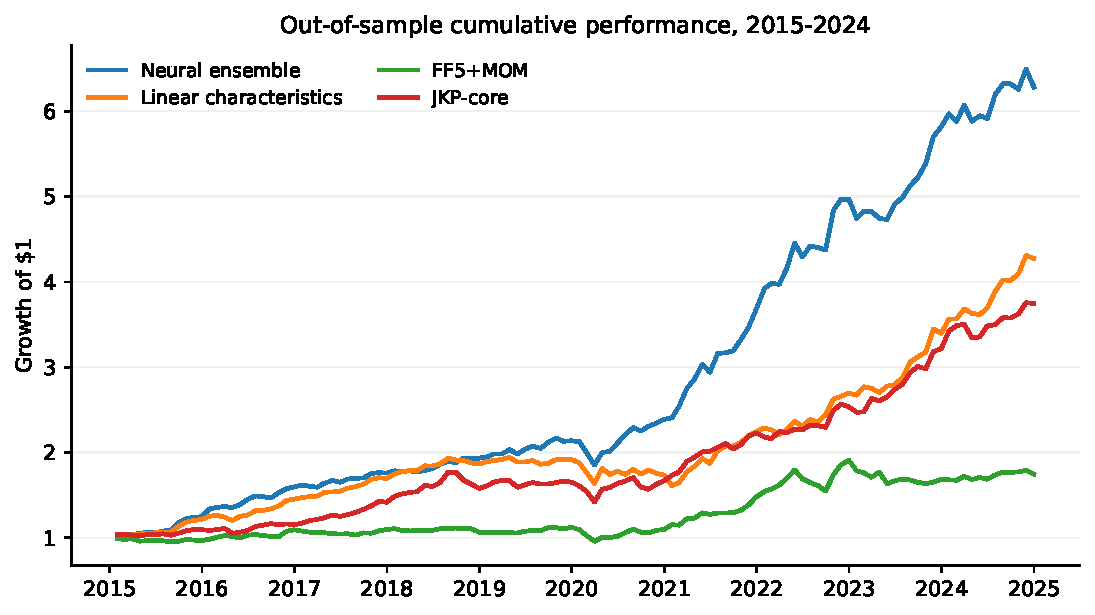
\includegraphics[width=0.88\textwidth]{figures/equity_flagship.pdf}
\caption{Out-of-sample cumulative performance, 2015--2024. For visual comparability only, each line is rescaled ex post to 10\% annualized volatility; this rescaling leaves Sharpe ratios unchanged. The neural line is the equal-weighted ensemble of ten $K_{\max}=32$ runs. Benchmark tangency weights are estimated before 2015.}
\label{fig:equityflagship}
\end{figure}

\begin{figure}[t]
\centering
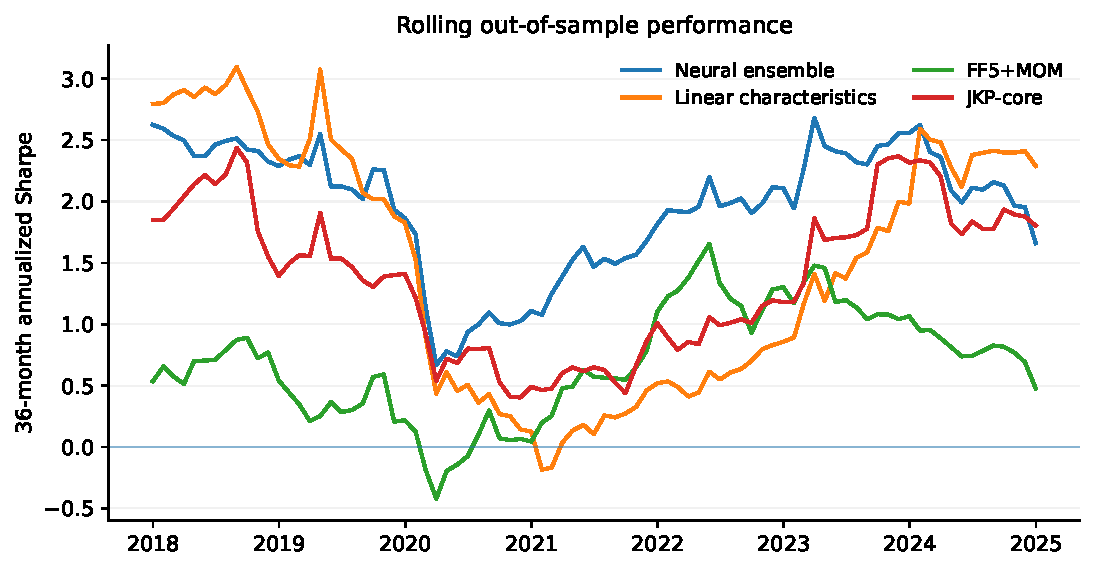
\includegraphics[width=0.88\textwidth]{figures/rolling_sharpe.pdf}
\caption{Thirty-six-month rolling out-of-sample Sharpe ratios. The figure shows whether performance is persistent through time rather than concentrated in one episode.}
\label{fig:rollingsharpe}
\end{figure}

\begin{figure}[t]
\centering
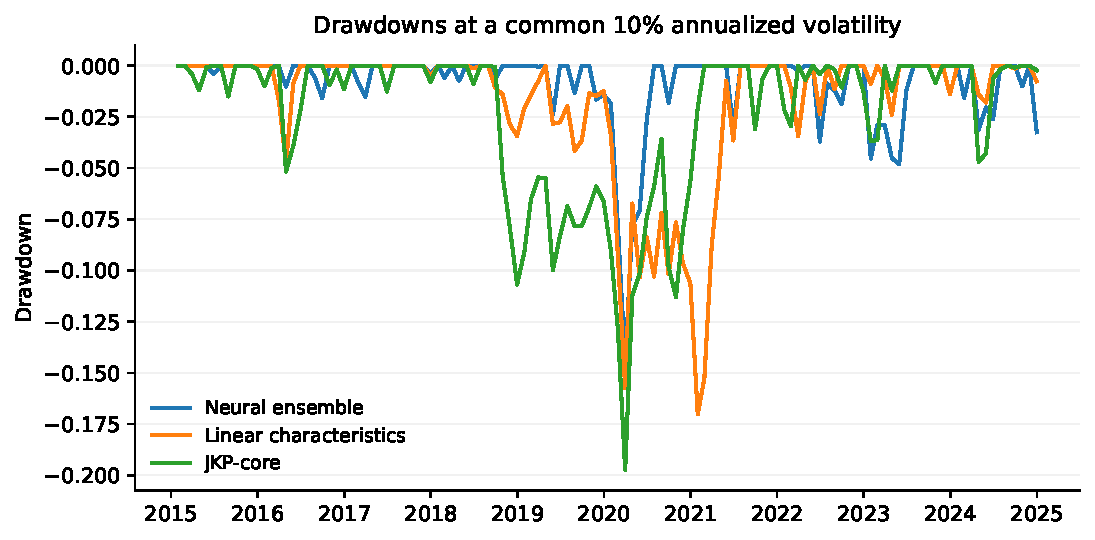
\includegraphics[width=0.86\textwidth]{figures/drawdown.pdf}
\caption{Out-of-sample drawdowns at a common 10\% annualized volatility. Volatility matching is applied ex post and only facilitates comparison of the path of losses across strategies.}
\label{fig:drawdown}
\end{figure}

The model is not designed to forecast every stock accurately. Its object is the portfolio payoff. This distinction matters empirically: improvements in the portfolio can arise from learning a stable ranking of economically useful characteristic combinations even when individual monthly stock returns remain mostly unpredictable.

\subsection{Nominal versus economic factor dimension}
The first main result is a sharp compression of the learned portfolio rule. Although the baseline architecture allows $K_{\max}=32$ latent factor coordinates, the rotation-invariant policy spectrum is strongly concentrated. The entropy policy dimension is \KEff, and the first policy direction accounts for \FirstShare\ of total spectrum mass. Figure~\ref{fig:spectrum} shows both the leading eigenvalues and their cumulative share.
\begin{figure}[t]
\centering
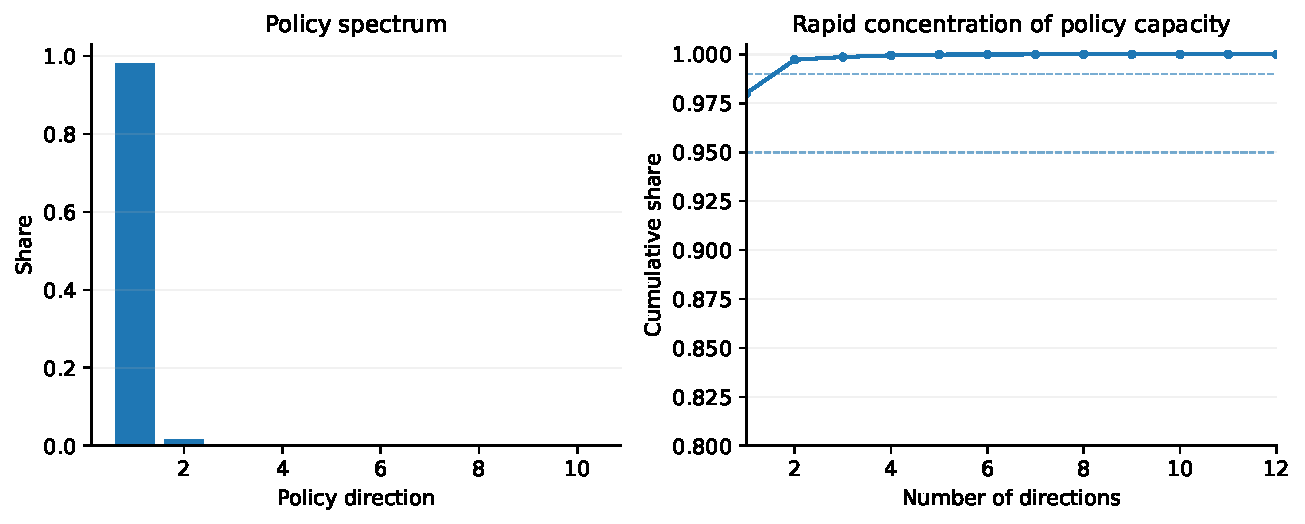
\includegraphics[width=0.86\textwidth]{figures/policy_spectrum.pdf}
\caption{Policy spectrum of the learned stock-weight rule. The left panel reports the leading normalized eigenvalues of the rotation-invariant policy operator; the right panel reports cumulative spectrum mass. The spectrum measures effective separable characteristic-by-state complexity, not the number of equilibrium risk factors.}
\label{fig:spectrum}
\end{figure}

Low policy dimension is not only a spectral statement. We also truncate the canonical traded-factor representation out of sample. With only two canonical directions, the reconstructed portfolio has a correlation of 0.997 with the full portfolio and a relative payoff MSE of 0.53\%; its Sharpe ratio is 1.68, essentially the same as the full representative model. Figure~\ref{fig:truncation} shows how rapidly the economic payoff is recovered as directions are added.
\begin{figure}[t]
\centering
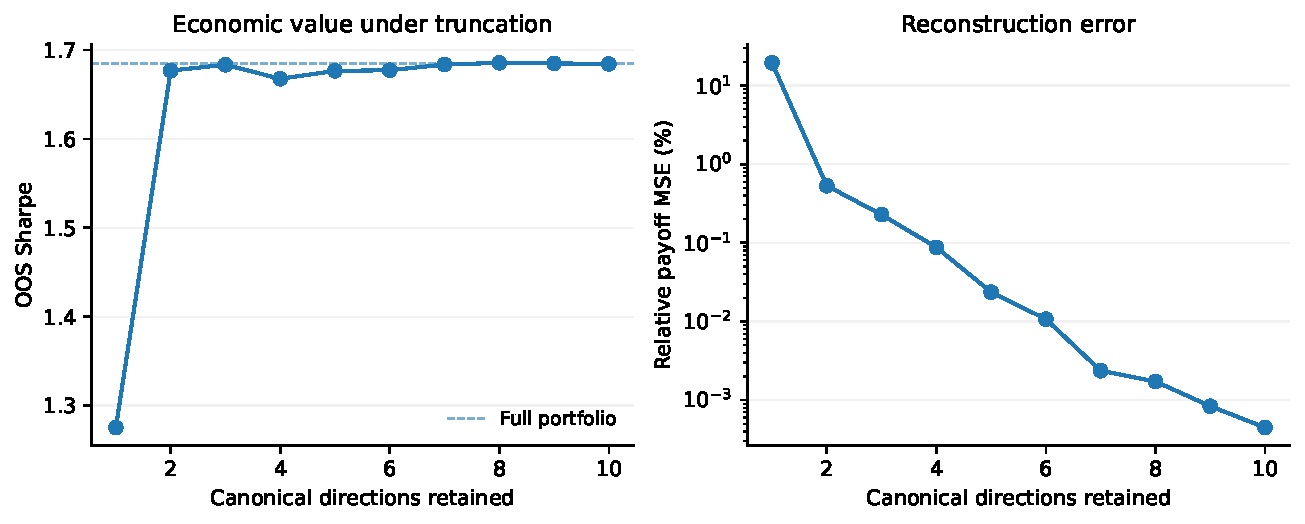
\includegraphics[width=0.86\textwidth]{figures/truncation.pdf}
\caption{Out-of-sample truncation of the canonical traded-factor representation. The left panel reports Sharpe as canonical directions are retained; the right panel reports relative payoff mean-squared error on a logarithmic scale.}
\label{fig:truncation}
\end{figure}

The distinction between nominal capacity and economic dimension is therefore useful. A network can use many parameters to synthesize nonlinear characteristic interactions while the final investment rule remains close to a very low-rank policy. Rich functional approximation and parsimonious economic structure are complements rather than substitutes.

The $K$-sweep makes this point directly. Table~\ref{tab:kgrid} uses the full 1963--2004 training sample, 2005--2014 validation sample, and 2015--2024 evaluation sample. Mean holdout Sharpe rises from 1.43 at $K_{\max}=1$ to 1.79 at $K_{\max}=32$, while the mean allocation rank rises only from 1.00 to 1.36. Thus additional representational capacity is useful for synthesizing better characteristic interactions, but it does not translate one-for-one into additional economically active portfolio directions.

\begin{table}[t]
\centering
\caption{Maximum Factor Capacity and Economic Dimension}\label{tab:kgrid}
\begin{threeparttable}
\begin{tabular}{rrrrr}
\toprule
$K_{\max}$ & Mean Test SR & SD & Ensemble SR & Allocation Rank \\
\midrule
1 & 1.43 & 0.10 & 1.51 & 1.00 \\
2 & 1.61 & 0.23 & 1.74 & 1.23 \\
4 & 1.69 & 0.21 & 1.87 & 1.21 \\
8 & 1.72 & 0.15 & 1.87 & 1.34 \\
16 & 1.72 & 0.17 & 1.89 & 1.33 \\
32 & 1.79 & 0.17 & 1.90 & 1.36 \\
\bottomrule
\end{tabular}
\begin{tablenotes}\footnotesize
\item Full-sample $K$ sweep: 1963--2004 training, 2005--2014 validation, 2015--2024 evaluation, ten random initializations per capacity. Ensemble returns equally average the ten model returns at each $K_{\max}$.
\end{tablenotes}
\end{threeparttable}

\end{table}

\begin{figure}[t]
\centering
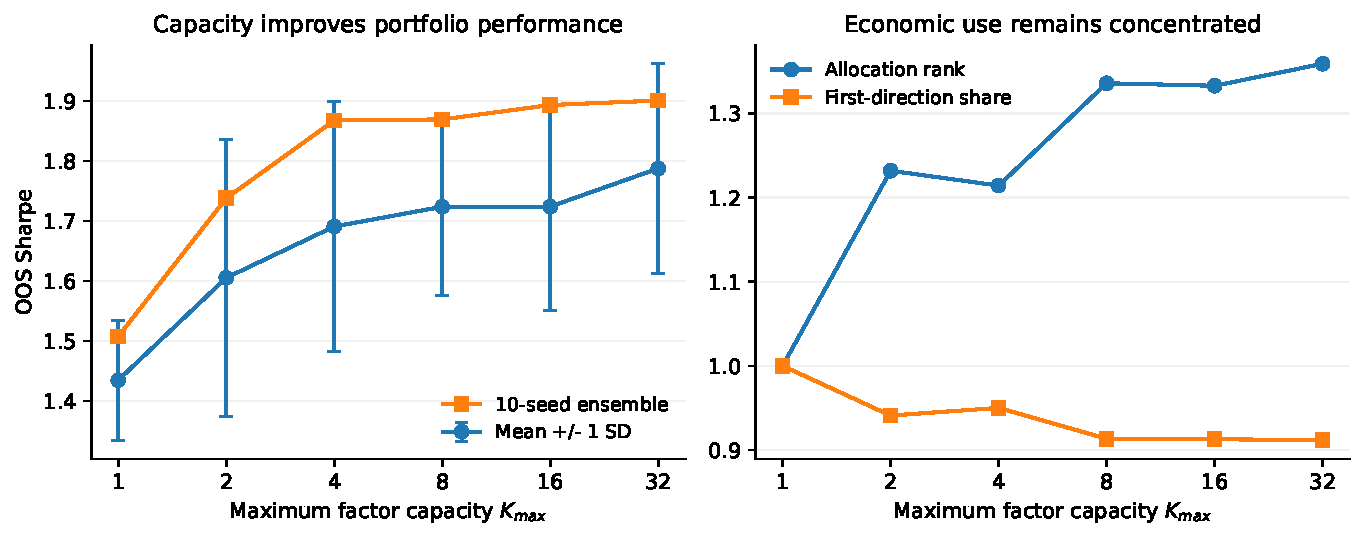
\includegraphics[width=0.92\textwidth]{figures/k_capacity.pdf}
\caption{Representation capacity and economic concentration. The left panel reports mean out-of-sample Sharpe across ten seeds and the corresponding seed ensemble for each $K_{\max}$. The right panel shows that allocation rank remains small even as nominal factor capacity increases.}
\label{fig:kcapacity}
\end{figure}

\section{What Does the Network Discover?}\label{sec:interpretation}
\subsection{The dominant characteristic factor}
The leading canonical factor has a clear economic profile, but it is not a standard one-dimensional sort. The factor places substantial weight on residual and conventional momentum, operating and cash profitability, earnings surprise, sales growth, and quality-related characteristics, while loading negatively on recent extreme winners. Table~\ref{tab:factorprofile} reports the largest characteristic sensitivities and top-minus-bottom characteristic spreads.
\begin{table}[t]
\centering
\caption{Economic Profile of the Dominant Learned Factor}\label{tab:factorprofile}
\begin{threeparttable}
\begin{tabular}{lrlr}
\toprule
Sensitivity characteristic & Share & Portfolio-tilt characteristic & Top--Bottom \\
\midrule
ret\_1\_0 & 2.45\% & mispricing\_mgmt & +0.46 \\
niq\_at\_chg1 & 2.19\% & fcf\_me & +0.45 \\
rmax5\_rvol\_21d & 2.17\% & mispricing\_perf & +0.42 \\
op\_at & 1.99\% & rmax5\_21d & -0.41 \\
seas\_1\_1an & 1.84\% & ocf\_me & +0.41 \\
ebit\_bev & 1.74\% & ebitda\_mev & +0.41 \\
market\_equity & 1.68\% & ocf\_at & +0.40 \\
lnoa\_gr1a & 1.66\% & ebit\_bev & +0.39 \\
rmax5\_21d & 1.66\% & rmax1\_21d & -0.38 \\
inv\_gr1 & 1.61\% & qmj\_prof & +0.38 \\
\bottomrule
\end{tabular}
\begin{tablenotes}\footnotesize\item Left columns report gradient sensitivity of the first canonical factor score. Right columns report the largest average top-decile minus bottom-decile characteristic ranks of the factor-sorted portfolio. These are descriptive diagnostics, not structural coefficients.\end{tablenotes}
\end{threeparttable}

\end{table}

\begin{figure}[t]
\centering
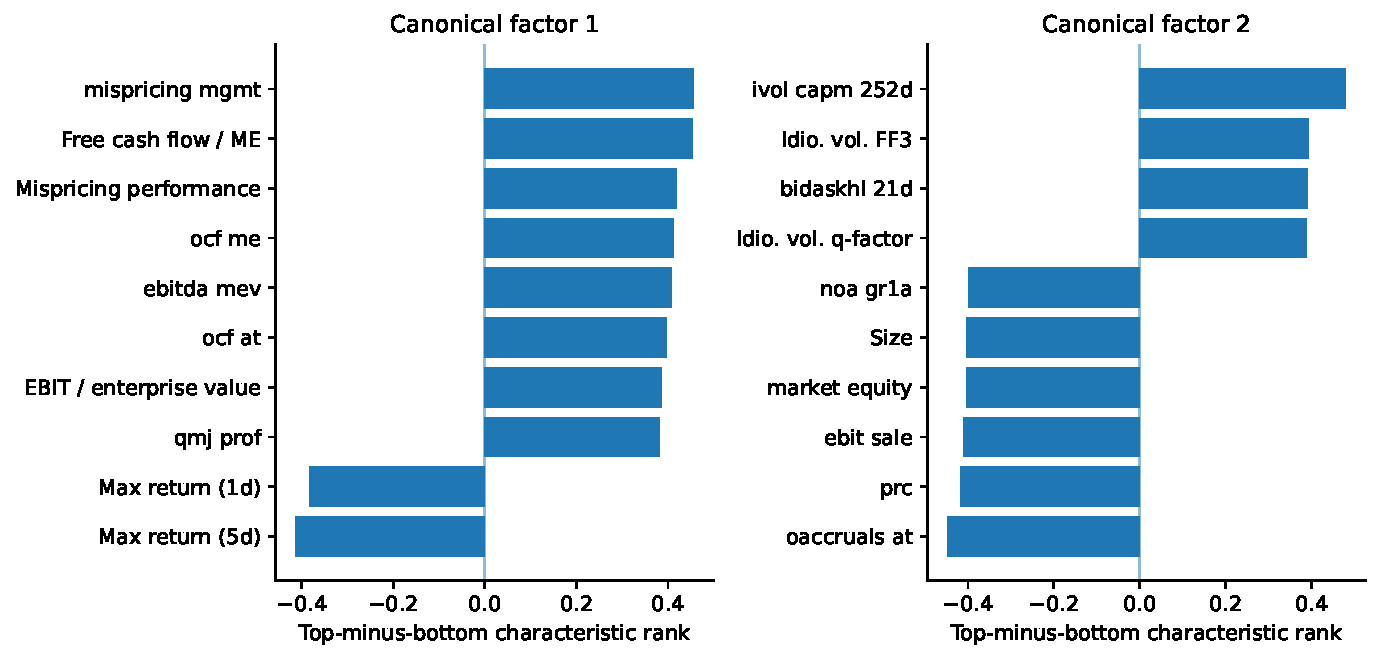
\includegraphics[width=0.92\textwidth]{figures/factor_profiles.pdf}
\caption{Economic profiles of the first two canonical learned factors. Bars report average top-decile minus bottom-decile characteristic ranks in the evaluation sample. The first direction combines quality and cash-flow strength with avoidance of extreme recent winners; the second loads on a distinct size, volatility, and investment configuration.}
\label{fig:factorprofiles}
\end{figure}

A useful summary is that the factor rewards stocks with persistent return strength supported by operating quality and fundamental news, while avoiding stocks whose apparent momentum is concentrated in a small number of extreme recent return days. This interpretation is deliberately descriptive: the learned score is a nonlinear function of all characteristics and cannot be reduced to a fixed additive factor recipe.

\subsection{Characteristic interactions}
The predictive content of the network does not come only from reweighting individual characteristics. We measure pairwise nonlinear interactions by jointly permuting two characteristics within a monthly cross-section and comparing the resulting change in the canonical factor score to the sum of the two separate permutation effects. The diagnostic preserves each month's empirical distribution and therefore tests whether the factor responds to a characteristic pair beyond the two marginal effects.

The largest interactions involve residual momentum with short-horizon returns, earnings surprise, extreme-return measures, and sales growth, together with interactions between short-horizon returns and earnings news. Figure~\ref{fig:interactions} displays the strongest pairs. The finding is consistent with the broader machine-learning evidence that nonlinear interactions account for an important part of cross-sectional predictability \citep{gu2020empirical}, but here the interactions are selected according to their value in the final tangency portfolio.

\begin{figure}[t]
\centering
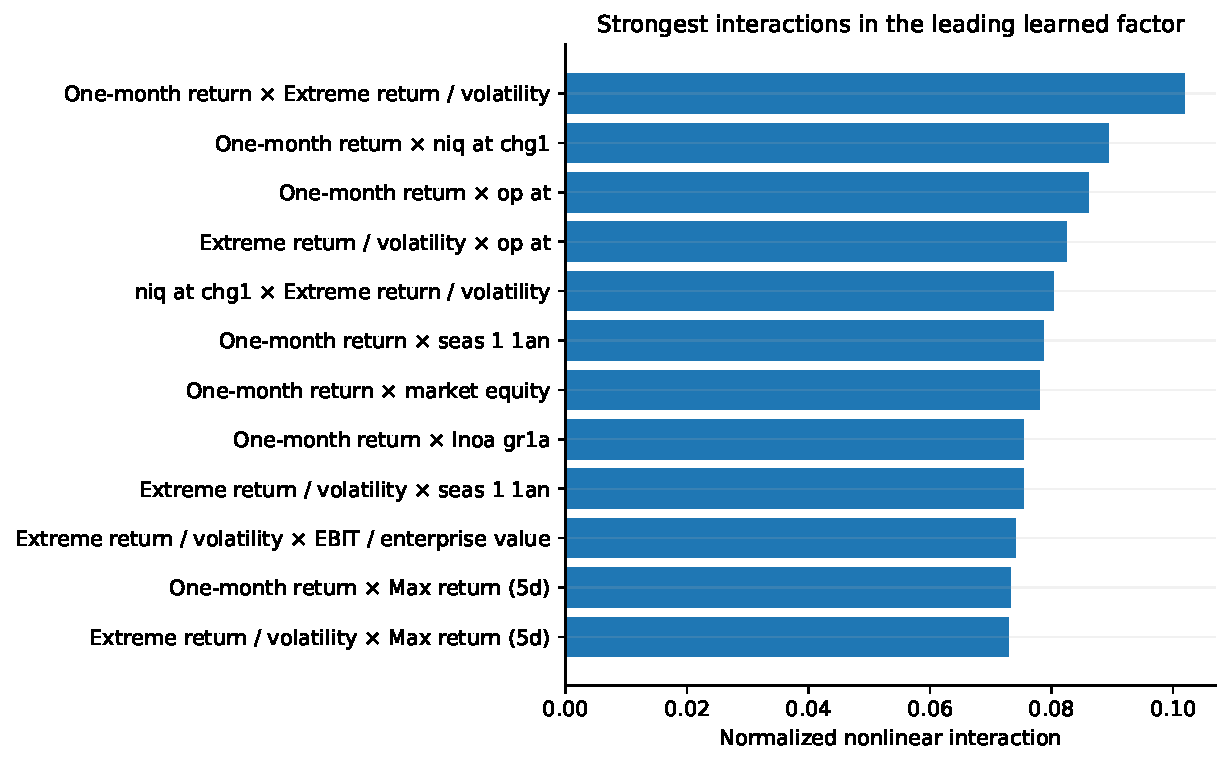
\includegraphics[width=0.82\textwidth]{figures/interactions.pdf}
\caption{Largest nonlinear characteristic interactions in the dominant canonical factor.}
\label{fig:interactions}
\end{figure}
\subsection{Conditional allocation}
The network separately learns when to hold the characteristic factor. The allocation to the leading factor varies with both aggregate market conditions and the learned cross-sectional state. In the baseline estimates, exposure falls materially when lagged market volatility and cross-sectional return dispersion are high and rises in stronger medium-horizon market states. This behavior is learned without assigning economic signs to the state variables ex ante.

This decomposition provides a finance interpretation of the neural network that a direct stock-level black box does not. The cross-sectional map answers which stocks express a factor; the allocator answers when that factor belongs in the tangency portfolio. The distinction also allows us to test whether the factor itself is stable even when its optimal exposure varies over time.

\begin{figure}[t]
\centering
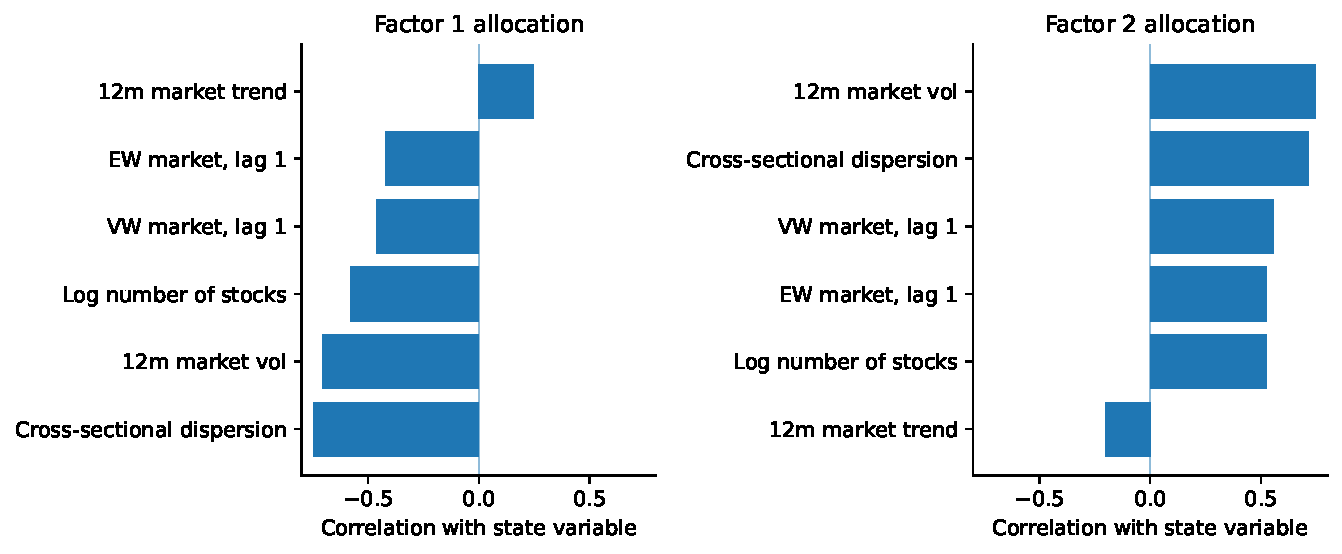
\includegraphics[width=0.92\textwidth]{figures/state_dependence.pdf}
\caption{State dependence of canonical factor allocations. Bars are correlations between factor allocations and lagged aggregate or cross-sectional state variables. They are descriptive of the learned conditional policy and are not causal estimates.}
\label{fig:state}
\end{figure}

\section{Spanning and Economic Value}\label{sec:spanning}
\subsection{Does the learned factor survive known models?}
A new characteristic combination is economically interesting only if it adds something beyond existing factor models. We therefore normalize the leading canonical factor to a 10\% annual volatility using only pre-test data and run time-series spanning regressions in the holdout period. Standard errors are Newey--West with six lags.

Table~\ref{tab:spanning} reports alphas relative to Fama--French five factors plus momentum, $q^5$, QMJ, the two JKP mispricing factors, and a broader JKP factor set. The test-period alpha remains positive across specifications. The Fama--French-plus-momentum alpha has a Newey--West $t$-statistic of \FFAlphaT, while the broad JKP specification yields a $t$-statistic of \JKPAlphaT.

\begin{table}[t]
\centering
\caption{Spanning Regressions for the Dominant Learned Factor}\label{tab:spanning}
\begin{threeparttable}
\begin{tabular}{lrrrr}
\toprule
Benchmark & Ann. Alpha & NW $t$ & $R^2$ & Hedged SR \\
\midrule
FF5 + MOM & 8.6\% & 4.97 & 0.75 & 1.48 \\
$q^5$ & 8.4\% & 3.32 & 0.56 & 1.07 \\
QMJ & 7.0\% & 2.15 & 0.56 & 1.31 \\
Mispricing-JKP & 4.9\% & 2.43 & 0.67 & 1.12 \\
JKP core & 5.7\% & 3.54 & 0.80 & 1.39 \\
\bottomrule
\end{tabular}
\begin{tablenotes}\footnotesize\item The learned factor is scaled to 10\% annual volatility using only pre-test data. Newey--West standard errors use six lags. Hedge coefficients are estimated before 2015 and applied in the evaluation period.\end{tablenotes}
\end{threeparttable}

\end{table}

\begin{figure}[t]
\centering
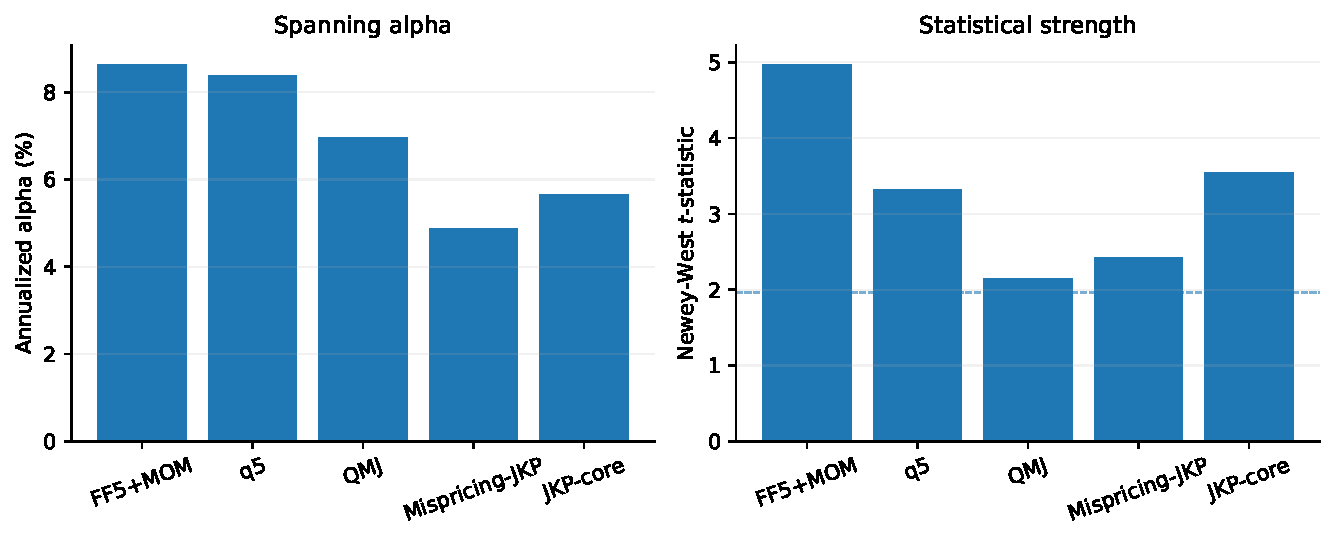
\includegraphics[width=0.90\textwidth]{figures/spanning_alpha.pdf}
\caption{Spanning evidence for the dominant learned factor. The left panel reports annualized evaluation-period alphas; the right panel reports Newey--West $t$-statistics, with 1.96 shown as a reference line.}
\label{fig:spanningalpha}
\end{figure}

The same conclusion appears when the known-factor exposures are estimated before the test period and hedged out in the holdout sample. The residual learned factor retains a positive Sharpe ratio across benchmark models. This exercise is stronger than a contemporaneous correlation comparison: it asks whether the historical exposures to known factors can eliminate the subsequent investment value of the learned direction.

\begin{figure}[t]
\centering
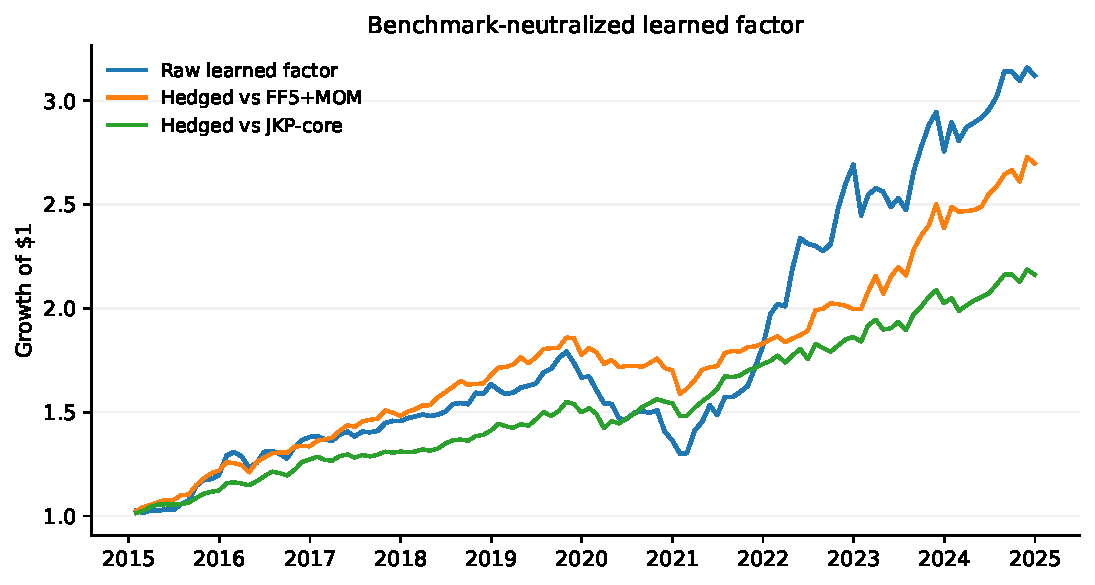
\includegraphics[width=0.86\textwidth]{figures/residual_equity.pdf}
\caption{Cumulative performance of the learned factor before and after neutralizing pre-2015 exposures to FF5+MOM and the broad JKP benchmark. Hedge coefficients are estimated before the evaluation sample.}
\label{fig:residualequity}
\end{figure}

\subsection{Marginal Sharpe}
For an asset manager, the relevant question is not whether a factor has a high standalone Sharpe ratio, but whether it improves an existing portfolio. We therefore estimate static tangency weights for each benchmark factor set using the pre-test sample and apply those weights to the holdout period. We then repeat the exercise after adding the learned factor. The change in realized holdout Sharpe is the factor's marginal portfolio value.

Across the benchmark sets, the learned factor increases the realized Sharpe of the pre-test tangency portfolio. Relative to the broad JKP benchmark, the increase is \MarginalSharpe. This result is directly relevant for a systematic investor: the network is not merely rediscovering a profitable factor in a new coordinate system; it finds a direction that improves a portfolio already containing major known sources of cross-sectional return variation.

\begin{table}[t]
\centering
\caption{Out-of-Sample Marginal Sharpe}\label{tab:marginal}
\begin{threeparttable}
\begin{tabular}{lrrr}
\toprule
Benchmark & Benchmark SR & + Learned Factor SR & Marginal SR \\
\midrule
FF5 + MOM & -- & -- & -- \\
$q^5$ & -- & -- & -- \\
QMJ & -- & -- & -- \\
Mispricing & -- & -- & -- \\
JKP core & -- & -- & -- \\
\bottomrule
\end{tabular}
\begin{tablenotes}\footnotesize\item Tangency weights are estimated before 2015 and evaluated in the 2015--2024 holdout sample.\end{tablenotes}
\end{threeparttable}

\end{table}

\begin{figure}[t]
\centering
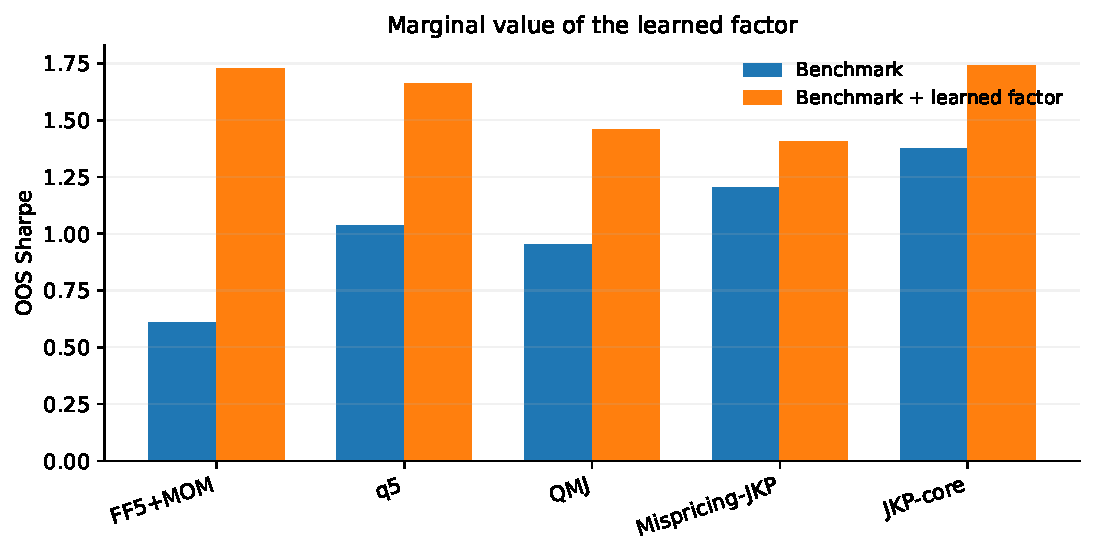
\includegraphics[width=0.84\textwidth]{figures/marginal_sharpe.pdf}
\caption{Marginal out-of-sample portfolio value. For each benchmark set, bars compare the Sharpe ratio of the pre-2015 estimated tangency portfolio with the Sharpe after adding the learned factor.}
\label{fig:marginalsharpe}
\end{figure}

\subsection{Turnover and trading costs}
High gross Sharpe ratios can be economically irrelevant when they require excessive trading \citep{novymarx2016taxonomy,jensen2026implementable}. We therefore examine the learned portfolio after lagged volatility scaling and proportional transaction costs. Table~\ref{tab:costs} reports turnover, gross exposure, and net performance. At 10 basis points per dollar traded, the annualized Sharpe is \NetSharpeTen.
\begin{table}[t]
\centering
\caption{Turnover, Volatility Scaling, and Transaction Costs}\label{tab:costs}
\begin{threeparttable}
\begin{tabular}{lrrr}
\toprule
Specification & Ann. Mean & Ann. Vol & Sharpe \\
\midrule
Gross, 10\% vol target & 18.7\% & 11.5\% & 1.63 \\
5 bps & 17.8\% & 11.5\% & 1.55 \\
10 bps & 16.8\% & 11.5\% & 1.46 \\
25 bps & 13.8\% & 11.5\% & 1.20 \\
10 bps + 100 bps borrow & 15.5\% & 11.5\% & 1.35 \\
10 bps + 300 bps borrow & 12.9\% & 11.5\% & 1.12 \\
\bottomrule
\end{tabular}
\begin{tablenotes}\footnotesize\item Volatility scaling uses lagged 36-month realized volatility and is not part of training. Average half-$L^1$ monthly turnover is 0.82 and average gross exposure is 2.81 in this representative run.\end{tablenotes}
\end{threeparttable}

\end{table}

\begin{figure}[t]
\centering
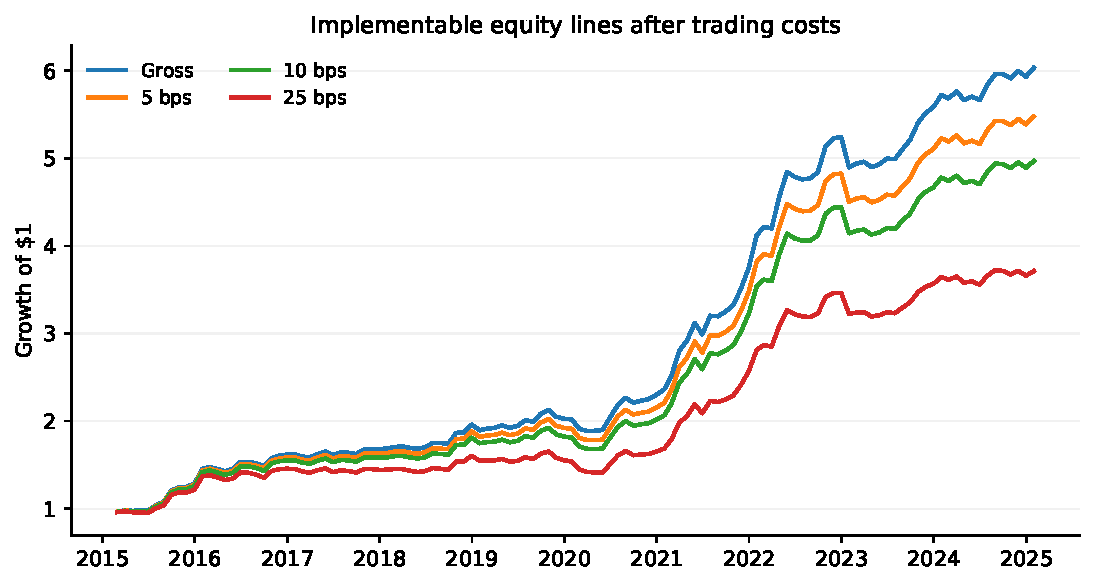
\includegraphics[width=0.86\textwidth]{figures/equity_costs.pdf}
\caption{Evaluation-period cumulative wealth after implementation costs. The representative neural portfolio is first scaled using lagged volatility and then charged one-way proportional trading costs of 5, 10, or 25 basis points per dollar traded.}
\label{fig:costequity}
\end{figure}

We view this exercise as a diagnostic rather than a claim that the frictionless network is cost optimal. A production strategy would optimally include costs in the training objective, as emphasized by \citet{jensen2026implementable}. Our question is narrower: whether the factor discovered from the frictionless tangency objective represents a sufficiently persistent source of return to remain economically relevant after ordinary trading frictions.

\section{Robustness and Walk-Forward Evidence}\label{sec:robustness}
\subsection{Random initialization and factor capacity}
Neural networks introduce optimization randomness, so a finance result should not depend on a favorable seed. We re-estimate each $K_{\max}\in\{1,2,4,8,16,32\}$ specification using at least ten random initializations. We report the mean, median, and dispersion of holdout Sharpe ratios together with the corresponding economic dimensions. The main conclusions are based on these distributions rather than on the single best run.

The $K$-grid separates approximation capacity from economic usage. If larger $K_{\max}$ only adds redundant coordinates, validation and evaluation performance should flatten. If it lets the network synthesize better nonlinear characteristic combinations, performance can continue to improve even when the effective policy and allocation ranks remain far below $K_{\max}$. The latter pattern is particularly informative: a high-capacity representation can be valuable without implying a high-dimensional implemented portfolio.

\begin{figure}[t]
\centering
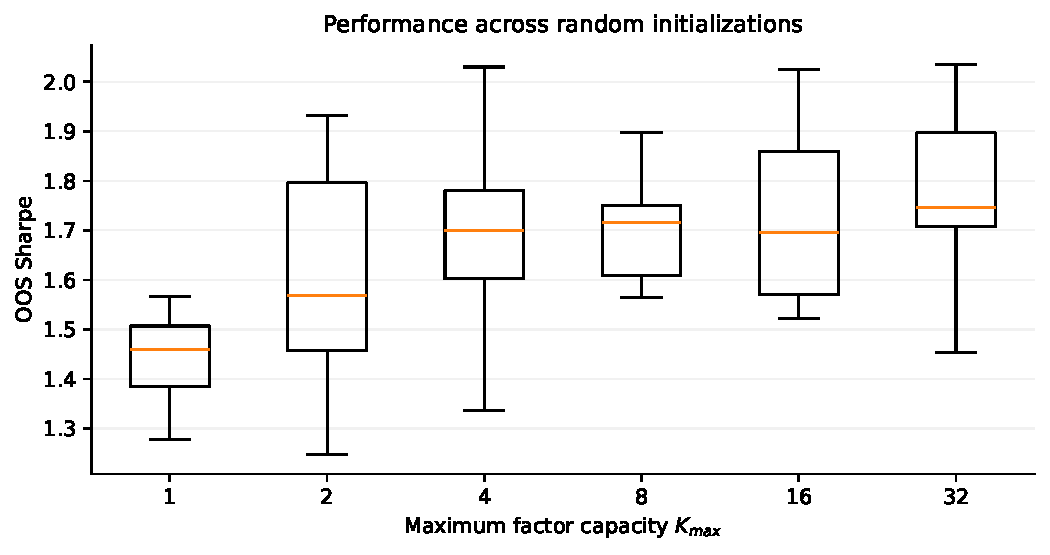
\includegraphics[width=0.78\textwidth]{figures/seed_dispersion.pdf}
\caption{Distribution of out-of-sample Sharpe ratios across ten random initializations at each factor capacity. The figure reports the full seed distribution rather than a best-seed backtest.}
\label{fig:seeds}
\end{figure}

\subsection{Ablations}
We estimate five economically targeted ablations. Removing aggregate market state $M_t$ lowers mean evaluation Sharpe from 1.83 to 1.53, and forcing a static factor allocation lowers it further to 1.46. Thus conditional factor timing is economically important. By contrast, removing the learned cross-sectional pooling block does not reduce performance: its mean Sharpe is 1.86. The cross-sectional attention mechanism is therefore not the source of the main result and can be viewed as an optional enrichment rather than a necessary ingredient. Making the characteristic map linear lowers mean Sharpe to 1.71, while a direct conditional neural stock policy without the factor bottleneck also delivers 1.71. The combination of nonlinear characteristic construction and a transparent conditional factor representation is therefore competitive with the less interpretable direct alternative.
\begin{table}[t]
\centering
\caption{Ablation Tests}\label{tab:ablations}
\begin{threeparttable}
\begin{tabular}{lrrr}
\toprule
Model & Mean Validation SR & Mean Test SR & Test SD \\
\midrule
Full factor model & 2.51 & 1.83 & 0.17 \\
No aggregate state $M_t$ & 2.55 & 1.53 & 0.17 \\
No cross-sectional pooling & 2.74 & 1.86 & 0.13 \\
Static factor allocation & 2.30 & 1.46 & 0.11 \\
Linear characteristic map & 2.74 & 1.71 & 0.04 \\
Direct conditional NN & 2.31 & 1.71 & 0.09 \\
\bottomrule
\end{tabular}
\begin{tablenotes}\footnotesize\item Five random initializations per specification. All models use the same 1963--2004 training and 2005--2014 validation samples and are evaluated over 2015--2024. No architecture is selected using test returns.\end{tablenotes}
\end{threeparttable}

\end{table}

\begin{figure}[t]
\centering
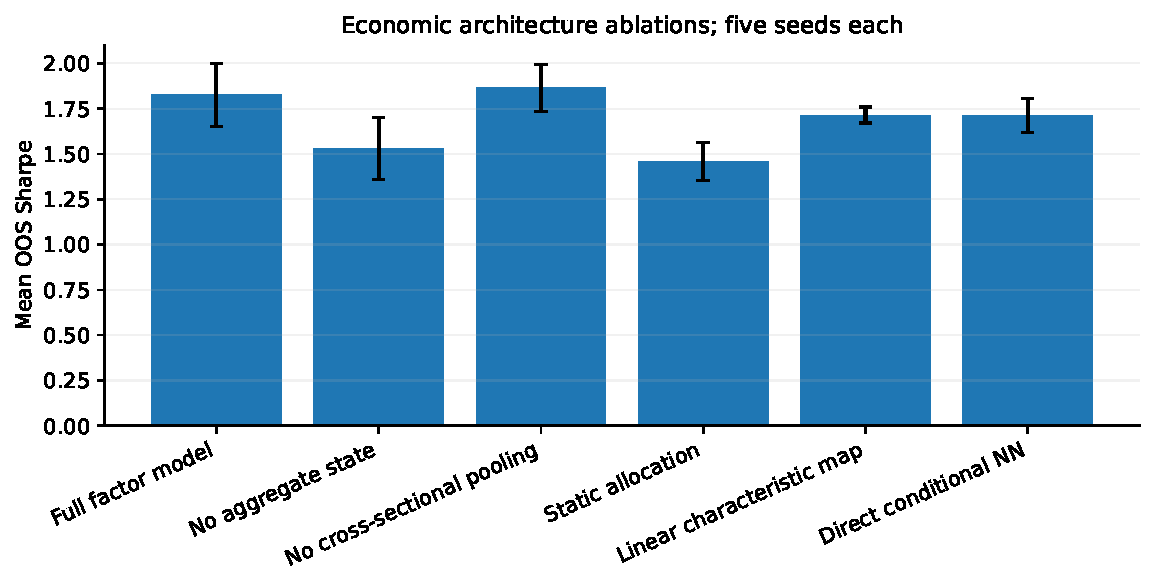
\includegraphics[width=0.84\textwidth]{figures/ablations.pdf}
\caption{Economic ablations. Bars report mean 2015--2024 Sharpe across five random initializations; error bars are one cross-seed standard deviation. The sharpest deterioration comes from removing aggregate state or making factor allocation static.}
\label{fig:ablations}
\end{figure}

\subsection{Expanding-window portfolio choice}
The fixed holdout protects against direct test-set tuning but still estimates one model before 2015. We therefore run a stricter annual walk-forward exercise. For each test year, the model uses an expanding history ending before the validation window, selects training progress using only the immediately preceding years, and then holds the resulting portfolio rule fixed throughout the next year. The procedure is repeated through 2024.

We repeat the full recursive exercise for five random initializations and average their monthly portfolio returns without using evaluation data to select a seed. The resulting walk-forward ensemble attains an annualized Sharpe ratio of \WalkForwardSharpe\ over 2015--2024; a 12-month circular-block bootstrap gives a 95\% interval of $[1.57,2.97]$. Individual recursive Sharpe ratios range from 1.24 to 2.23, with a mean of 1.97. A recursive linear-characteristic benchmark, re-estimated on the same expanding information set with its ridge penalty fixed before 2015, reaches Sharpe \WalkForwardLinearSharpe. The neural-minus-linear difference is \WalkForwardDelta\ Sharpe points; a paired 12-month block bootstrap gives $[-0.22,1.39]$, with 92\% of bootstrap draws positive. We therefore view the recursive improvement as economically substantial but not yet statistically decisive. The neural ensemble Sharpe is positive in every payoff year, including 2020. Figure~\ref{fig:walkforward} compares recursive neural and linear policies, together with the fixed-split neural ensemble. The exercise exposes the model to changing market composition, characteristic distributions, and aggregate states while ensuring that each year's payoff is generated by a rule estimated using only information available beforehand.

\begin{figure}[t]
\centering
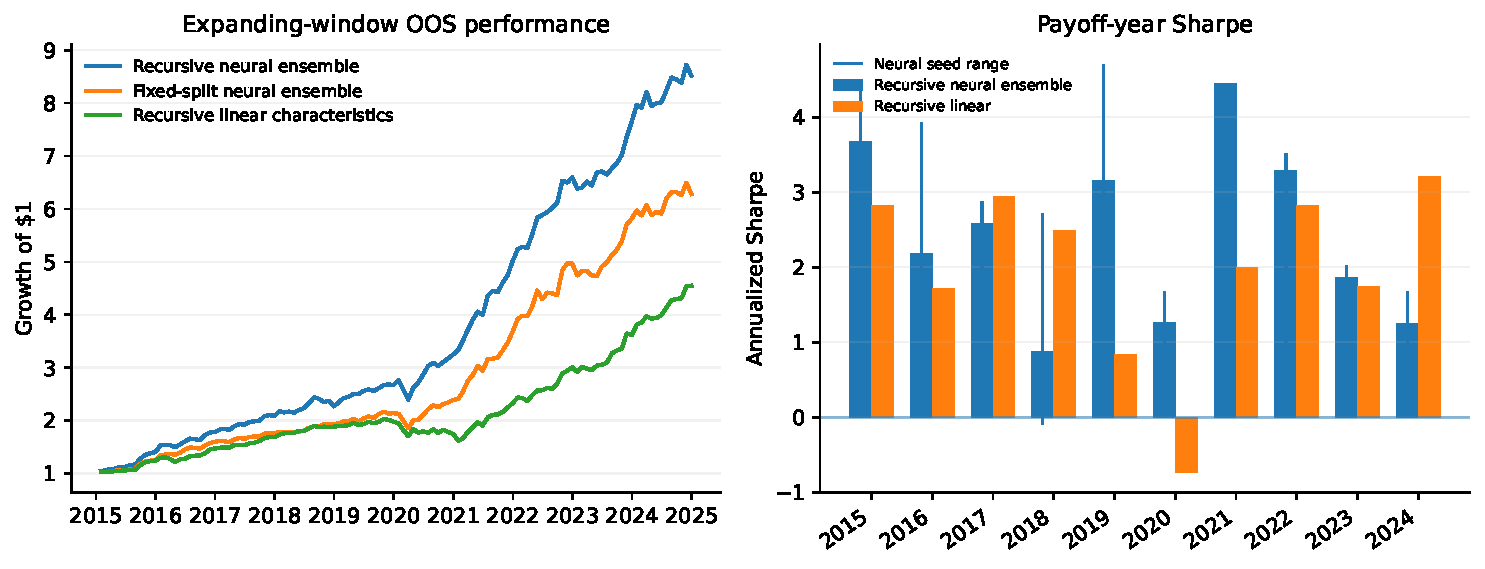
\includegraphics[width=0.90\textwidth]{figures/walk_forward.pdf}
\caption{Expanding-window walk-forward performance. Left: cumulative performance of the five-seed recursive neural ensemble, the fixed-split neural ensemble, and the recursively re-estimated linear-characteristic benchmark, each rescaled ex post to 10\% annualized volatility. Right: annualized Sharpe by payoff year for recursive neural and linear policies; vertical ranges span the five neural seeds. Every test-year portfolio is estimated before that payoff year begins.}
\label{fig:walkforward}
\end{figure}

\subsection{Stability of factor interactions and economic dimension}
We finally ask whether the dominant nonlinear factor is a stable economic object or a feature of one subperiod. We measure the canonical allocation rank separately in early training, late training, validation, and test samples. We also hold a common set of leading characteristics fixed and re-estimate pairwise interaction diagnostics within each subperiod.
The allocation remains concentrated throughout the sample. Interaction rankings are moderately related between the earliest training subsample and later periods, and become highly stable once the model reaches the late-training, validation, and evaluation eras. Table~\ref{tab:stability} reports allocation rank, the share of the first canonical direction, pairwise Spearman rank correlations, and overlap among the strongest interactions.

\begin{table}[t]
\centering
\caption{Stability of Economic Dimension and Characteristic Interactions}\label{tab:stability}
\begin{threeparttable}
\begin{tabular}{lrrr}
\toprule
Period & Allocation Rank & First Share & Top-2 Share \\
\midrule
Early training & 1.27 & 94.0\% & 99.8\% \\
Late training & 1.34 & 91.8\% & 99.8\% \\
Validation & 1.53 & 85.7\% & 99.8\% \\
Test & 1.63 & 81.9\% & 99.8\% \\
\bottomrule
\end{tabular}
\begin{tablenotes}\footnotesize\item The same trained $K_{\max}=32$ network is evaluated in each subperiod. Pairwise interaction-rank correlations are reported graphically in Figure~\ref{fig:interactionstability}.\end{tablenotes}
\end{threeparttable}

\end{table}

\begin{figure}[t]
\centering
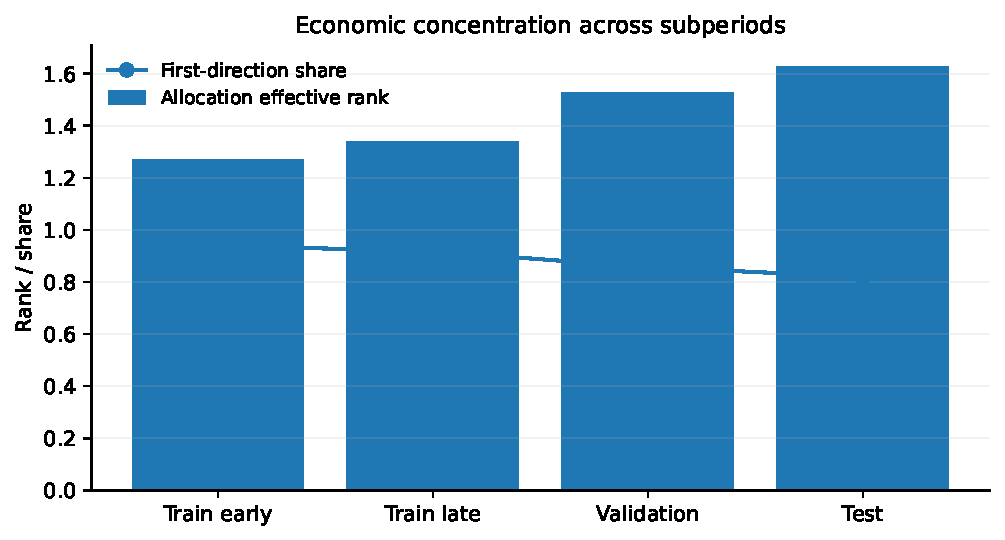
\includegraphics[width=0.76\textwidth]{figures/dimension_by_period.pdf}
\caption{Concentration of the canonical allocation across subperiods. The learned strategy remains low-dimensional even though the market environment and cross-sectional composition change materially over six decades.}
\label{fig:dimensionperiod}
\end{figure}

\begin{figure}[t]
\centering
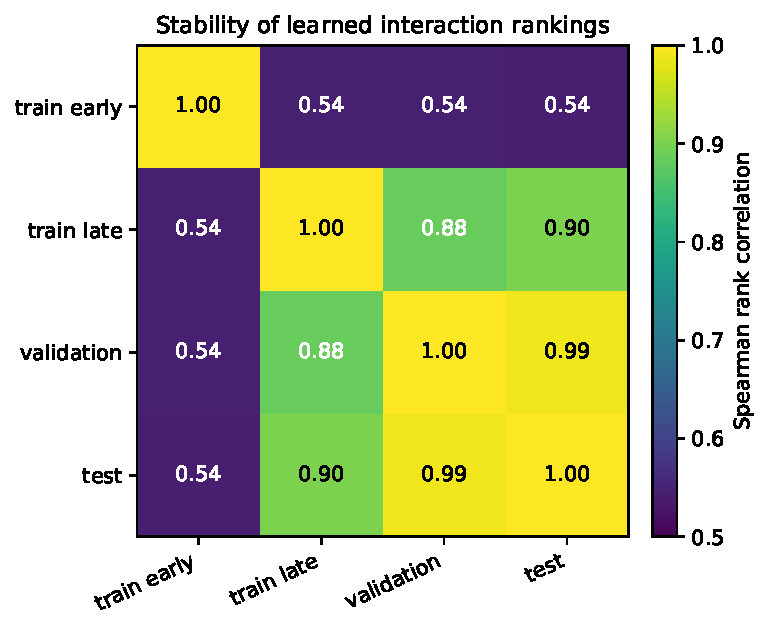
\includegraphics[width=0.66\textwidth]{figures/interaction_stability.pdf}
\caption{Stability of nonlinear interaction rankings across subperiods. Entries are Spearman rank correlations computed using a characteristic set fixed from training data.}
\label{fig:interactionstability}
\end{figure}

\section{Conclusion}\label{sec:conclusion}
The characteristic zoo is high-dimensional in observables, but portfolio choice need not be. This paper gives a neural network enough flexibility to combine a large characteristic set nonlinearly while forcing the final portfolio to operate through a transparent factor bottleneck. The resulting factors are not chosen by univariate sorts or by reconstruction of the return panel. They are chosen because they matter for the conditional tangency portfolio.

The main empirical message is a separation between statistical complexity and economic dimension. A richly parameterized network can use many characteristics and interactions while concentrating its portfolio on only a few risk-standardized factor directions. The leading direction combines momentum, profitability and quality, fundamental news, growth, and avoidance of extreme recent winners, and its desired exposure changes with market conditions. Standard factor models do not fully span the resulting investment opportunity.

For asset pricing, this finding suggests a different interpretation of the factor zoo. Many published characteristics may be useful not because each represents a separate factor, but because they provide ingredients for a smaller number of nonlinear characteristic combinations. For asset management, the same result suggests that feature learning can be used as factor discovery: the output of the network can be analyzed as a set of traded economic directions rather than as a black-box expected-return forecast.

Several extensions are natural. Transaction costs can be integrated directly into the learning objective, the factor map can be estimated jointly across countries, and the policy spectrum can be studied across asset classes. The central object, however, remains the same: the dimension and composition of the characteristic information that actually survives into the investor's portfolio.

\appendix
\section{Additional Details}
\subsection{Network architecture}
The stock encoder consists of fully connected layers with SiLU activations and layer normalization. The factor head produces $K$ nonlinear characteristic scores. Each score is normalized to unit cross-sectional root-mean-square as in \eqref{eq:score_normalization}. A learned attention pool produces a permutation-invariant cross-sectional state. The allocator maps this state together with lagged aggregate variables into $K$ factor positions.
\subsection{Optimization}
Training uses contiguous monthly blocks. Within a block $\mathcal{B}$, the loss is the negative sample analogue of \eqref{eq:tangency_score},
\[
-\frac{|\mathcal{B}|^{-1}\sum_{t\in\mathcal{B}}R^p_{t+1}}
{\left(|\mathcal{B}|^{-1}\sum_{t\in\mathcal{B}}(R^p_{t+1})^2+\varepsilon\right)^{1/2}}.
\]
This block objective supplies a time-series risk signal to every gradient update. Validation Sharpe determines learning-rate reductions and early stopping. The test sample is never used to select epochs, $K$, network width, or regularization.

\subsection{Spanning regressions}
For benchmark factor vector $B_{t+1}$, we estimate
\[
G_{1,t+1}=\alpha+\beta'B_{t+1}+\varepsilon_{t+1},
\]
where $G_1$ is the leading canonical learned factor scaled to 10\% annual volatility using pre-test data. We report Newey--West $t$-statistics with six lags. To construct the out-of-sample hedged factor, $\beta$ is estimated before the holdout period and only the factor hedge $\widehat\beta'B_{t+1}$ is subtracted in the test sample.

\subsection{Turnover}
Let $w_t$ denote the volatility-scaled target positions at month end. Previous holdings are allowed to drift with realized individual-stock returns before rebalancing. Dollar notional traded is the $\ell_1$ distance between current target positions and previous post-return holdings. A cost of $c$ basis points subtracts $c/10{,}000$ times dollar notional traded from the monthly portfolio return.

\section{Additional Empirical Figures}
The following figures document the time-series path, implementation burden, and factor decomposition behind the main results. They are included to make clear where the reported Sharpe ratios come from and whether the findings are concentrated in particular years or particular components of the learned strategy.

\begin{figure}[p]
\centering
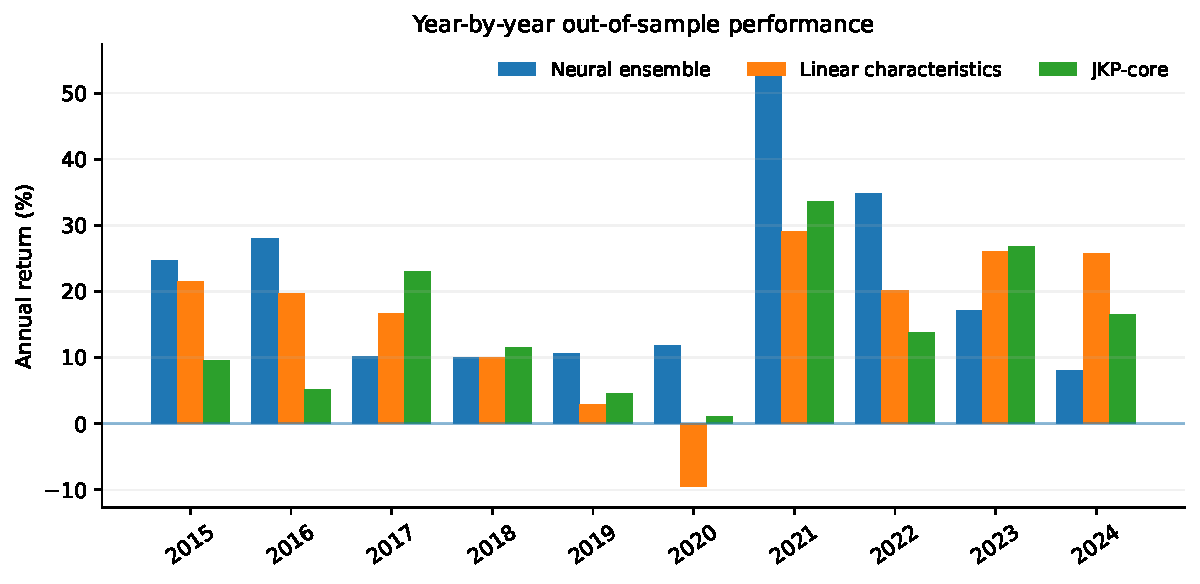
\includegraphics[width=0.90\textwidth]{figures/annual_returns.pdf}
\caption{Calendar-year evaluation-period returns at a common 10\% annualized volatility.}
\label{fig:annualreturns}
\end{figure}

\begin{figure}[p]
\centering
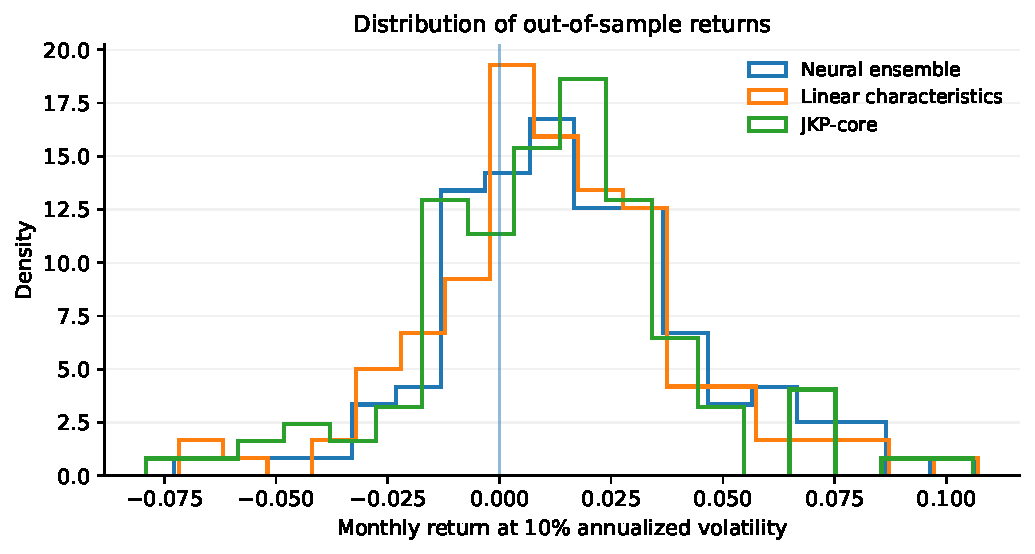
\includegraphics[width=0.84\textwidth]{figures/return_distribution.pdf}
\caption{Distribution of monthly evaluation-period returns for the neural ensemble, linear-characteristic benchmark, and broad JKP tangency portfolio, each rescaled ex post to common volatility.}
\label{fig:returndist}
\end{figure}

\begin{figure}[p]
\centering
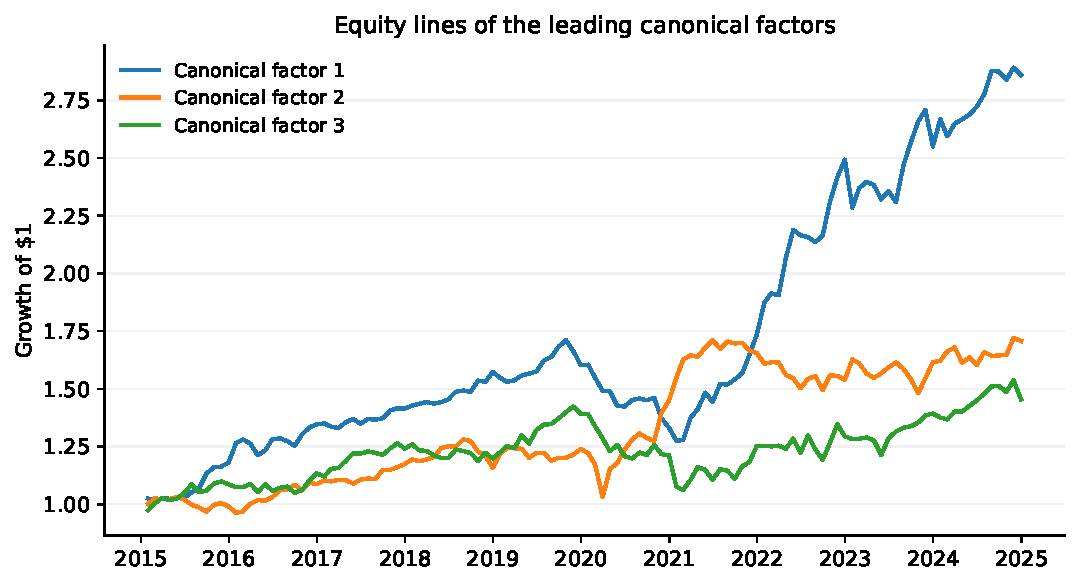
\includegraphics[width=0.88\textwidth]{figures/factor_equity.pdf}
\caption{Cumulative wealth of the leading canonical learned factors, each rescaled ex post to 10\% annualized volatility for visual comparison.}
\label{fig:factorequity}
\end{figure}

\begin{figure}[p]
\centering
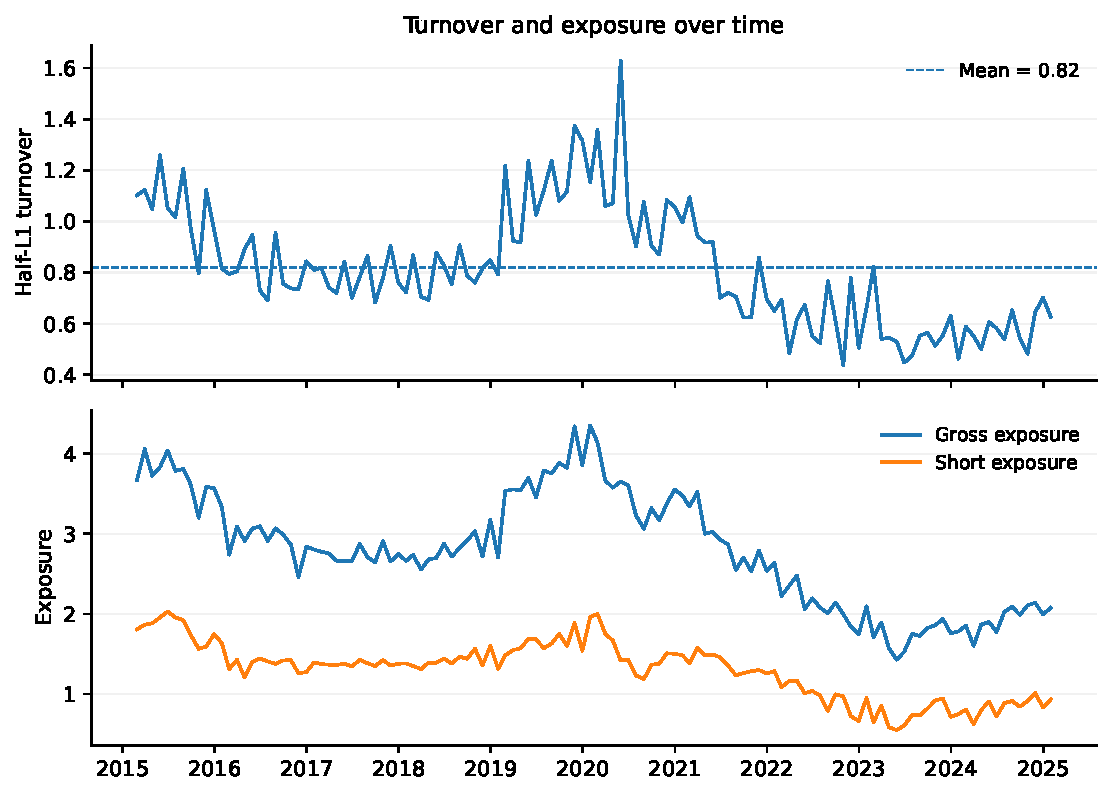
\includegraphics[width=0.88\textwidth]{figures/turnover_exposure.pdf}
\caption{Turnover and exposure of the representative learned portfolio through the evaluation sample.}
\label{fig:turnoverexposure}
\end{figure}

\begin{figure}[p]
\centering
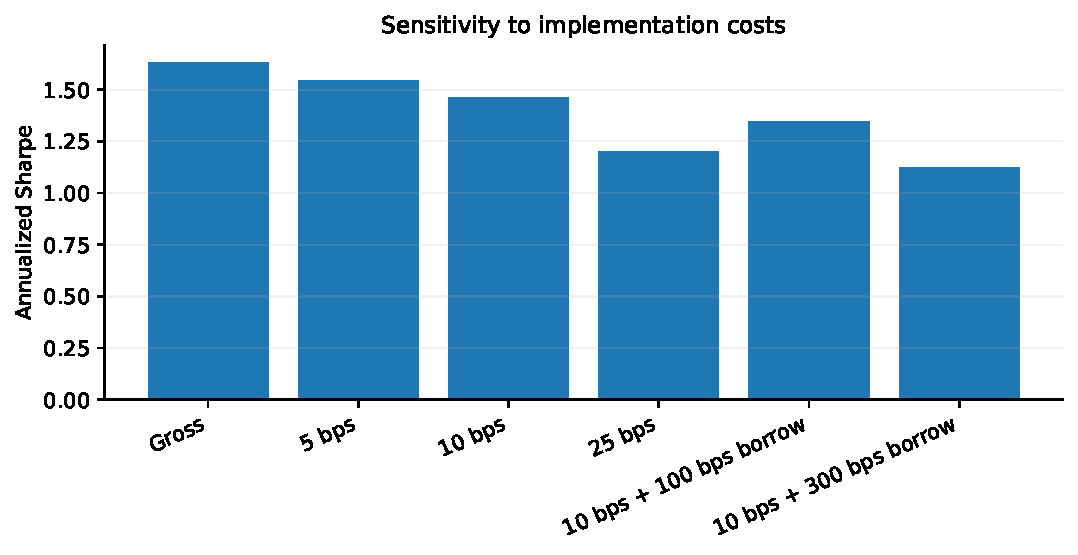
\includegraphics[width=0.82\textwidth]{figures/cost_sensitivity.pdf}
\caption{Sharpe ratio under alternative transaction-cost and short-borrow assumptions.}
\label{fig:costsensitivity}
\end{figure}

\bibliographystyle{apalike}
\bibliography{references}
\end{document}
